\section{Marketing}
In order to understand the special features of B2B marketing, in this chapter a fundamental overview of the marketing mix will be used to extract the relevant parts of marketing, that need to be considered for the conception of a application at it is desired. After showing the basic differences between B2B and consumer marketing, the impacts of these differences to the relevant part of the marketing mix will be described. In the end of this chapter the approach of market orientation for dealing with these specialties will be explained and described.
\subsection{Marketing Mix}
The term \textit{marketing mix} is be defined as the combination of different marketing instruments \parencite[cf.][285]{Thommen.2012}. There are  different categories of those instruments: originally described by \textcite[cf.][]{McCarthy.1993} the basic marketing mix, consisting of the so called \textit{4 Ps} "product, place, price, and promotion" \sekcite{McCarthy.1993}{}{Rafiq.1995}{}. This paper will use a more recent set of nomenclature, because it more precisely describes the contents of the categories. The recent naming maps place to \textit{distribution}, price to \textit{terms and conditions}, and promotion to \textit{communication}, while \textit{product} is not renamed \parencites[285]{Thommen.2012}[cf.][397-720]{Meffert.2015}. 
\paragraph*{} In addition to these points, even more recent approaches, also include the categories "participants [some times calles people; note from the author], physical evidence, and process" \parencite{Rafiq.1995}. \Cref{fig:aspects} shows all seven aspects.  and some examples for what they the individual categories including. This is not a complete list, but may help to minimize the likelihood of confusion. Beneath it, the categories are described with examples, and their link to the concept.

\begin{figure}[H]
	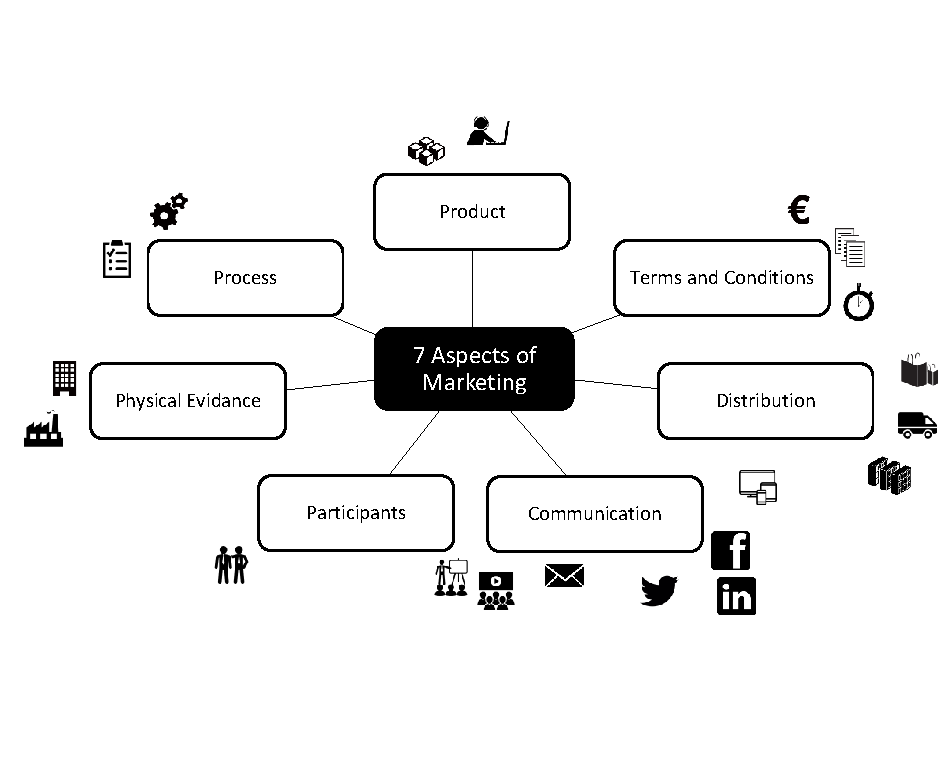
\includegraphics{img/7p.pdf}
	\caption[7 Aspects of Marketing]{The 7 Aspects of Marketing as used in this paper (own illustration based on \protect\cites[285]{Thommen.2012}[397-720]{Meffert.2015}{Hoepner2015})}
	\label{fig:aspects}
\end{figure}
\begin{enumerate}
    \item{Product:}The value of the individual product to be sold alone, and as part of the program of the selling company \parencite[cf.][398]{Meffert.2015}. As a example, the iPhone has certain features and specification. Additionally, it is part of the program of Apple, beside the iPad, several Mac Products and other things, including accessories and more. The individual product and its integration into the providers program can generate value to the customer, and different competitive advantages.
    \item{Terms and Conditions:}The terms and condition range from the price for purchase to service level agreements and warranty agreements, governing law, and many more. As an example, it is possible for several software products to be purchased with drastically different service levels tied to different prices. \\
    The contractual terms and conditions are negotiated by the customer and IBM for each case individually. Resulting from this, the desired application has no impact on this point, nor does it influence the desired instrument \parencite[cf.][]{Sachs.20.04.2017}.
    \item{Distribution:}The question of where and how you can purchase the product. For instance, it is possible to purchase the iPhone in a wide variety of stores, including Apple Stores, online, at most mobile service providers. On the other hand, the first One Plus was only available online and only by being invited by someone legitimate.\\
    The service sold, is by definition distributed as on-site, or remote service workers \parencite[cf.][]{Sachs.20.04.2017}. This as well cannot be influenced or changed by an pre-sales information application.
    \item{Communication:}This includes for example commercials, public relations, as well as sales men. \\
    The applications main goal is to build an additional channel of communication to the customer to explicitly show the technical competence of IBM. For that reason, the communication mix has a huge influence on the application, since it has to fit in an support other instruments of communication.
    \item{Participants:}The concrete individuals involved in placing the goods at the disposal. This includes for instance their skills and appearance. Someone dressed in a suit, may not be perceived as a creditable plumber. \\ 
    The participants of the service product can be different from each customer and project to the other. It may be possible to include information about the team in the application, which would underline the competence of each consultant.
    \item{Physical Evidence}
    \textcite[155]{AzilaGbettor2013} cite \textcite{Booms.1981} as describing the physical evidence, the physical environment surrounding the service. This explicitly targets the premises and related entities \parencite[cf.]{Hoepner2015}.
    \item{Process Parts:}
    The process parts describe the process of the contract fulfillment \parencite{Hoepner2015}.\\
    Thereby this has no direct influence on the pursed implementation. 
\end{enumerate}
\paragraph*{} As stated above, the outcome of this paper is connected to the communication, but as input for the design, the people and the product must be taken into account. 
\subsection{B2B versus B2C Marketing}
Several applications of the marketing instruments mentioned above are known from consumer market companies. Common examples PayPal's Terms and Conditions with their customer protection \parencite[see][]{PayPal}, the communication techniques of Apple etc.
\paragraph*{} \textcite[20-21]{Backhaus.2015b} states, that those consumer marketing and industrial marketing differ in several points.
\begin{table}[H]
\begin{center}
\begin{tabular}{|c|c|c|}
\hline 
 & Industrial Marketing & Consumer Marketing \\ 
\hline 
Demand & Derived & Direct \\ 
\hline 
Customers & Organizations & People \\ 
\hline 
Decision makers & Mainly multiple people & Mainly sole people \\ 
\hline 
Requirements & Formalized & Not formalized \\ 
\hline 
Market & Identified & Anonymous \\ 
\hline 
\end{tabular} 
\end{center}
\caption[Differences between industrial and consumer marketing]{Differences between industrial and consumer marketing (own illustration based on \protect\cite[21]{Backhaus.2015b})}
\label{tab:marketingdiff}
\end{table}
As to be seen in \Cref{tab:marketingdiff}, the circumstances for industrial - or B2B - marketing differ. It is worth taking a note, which points influence the conception of a marketing application as it is desired by this paper. 
\paragraph*{Demand:} The demand of a consumer market is by definition direct demand, since it is caused by a consumer wanting or needing something. The suppliers for the requested goods themselves require goods and services in order to fulfill the consumer needs. Therefore the B2B demand is derived from the direct demand \parencite[cf.][21]{Backhaus.2015b}. This implies, that one marketing strategy must be planned in respect to the downstream demand down to the consumer. 
\paragraph*{Customers:} Because organizations - not people - are the target customers in B2B marketing, the legal and organizational complexity must be considered, as explained in the following two points.
\paragraph*{Decision makers:}Regarding consumer purchases, the dominant part is decided on by an individual or a pair of two characters. Organizations on the other hand have larger groups of people involved in such a decision. This results in not only more people that have to be convinced, but also in differing target groups for the same product, e.g. the financial department, the technical department, and some operating department. 
\paragraph*{Requirements:}In consumer markets, suppliers try to anticipate the needs of the customers, and offer goods and services designed by these assumptions. In the B2B market this is still true for some products, in the specific field of this paper, customer companies define their requirements in their request for proposal. Therefore, it is possible to adapt the marketing mix to the individual case.
\paragraph*{Market:}In B2B markets, the supplier and customers are more likely to specifically know each other than in consumer good markets. For that reason, it id possible to identify needs in direct contact.
\paragraph*{} Those points can be linked directly linked to the point of communication. The benefits for communication in a B2B environment are  the direct contact between supplier and costumer, which generates the possibility for individualized communication approaches, and the formally described requirements, allowing direct referencing those. The downsides are larger decision groups are involved. They may be indirectly linked to the point of participants, since they are those in direct contact with the customer. They collect the lessons learned and formulate any technical information to be displayed in the desired application.
\paragraph*{}By the end of this section, all marketing related statements will relate to B2B marketing only.
\subsection{The Market Orientation Marketing Approach}
\textcite[9-10]{Claen.2016} shows that the term market orientation is used with a wide variety of definitions, from subjecting business to formulated customer demands only all the way to a complex orientation of business based on the complete market of the customer.
\begin{figure}[H]
	
\includegraphics[width=\textwidth]{img/supplychain.pdf}
	\caption[Supply Chain Schema]{Supply Chain Schema(own illustration based on \protect\cite{SouthwestTech})}
    	\label{fig:supplychain}
\end{figure}
The complete market in this context means the supply chain, as seen in \Cref{fig:supplychain}, and duties to all his stakeholders. \parencite[cf.][22-23]{Claen.2016}. A overview of the customers operational business at the center of his stakeholders, is sketched out in \Cref{fig:SGM}.
\begin{figure}[H]
	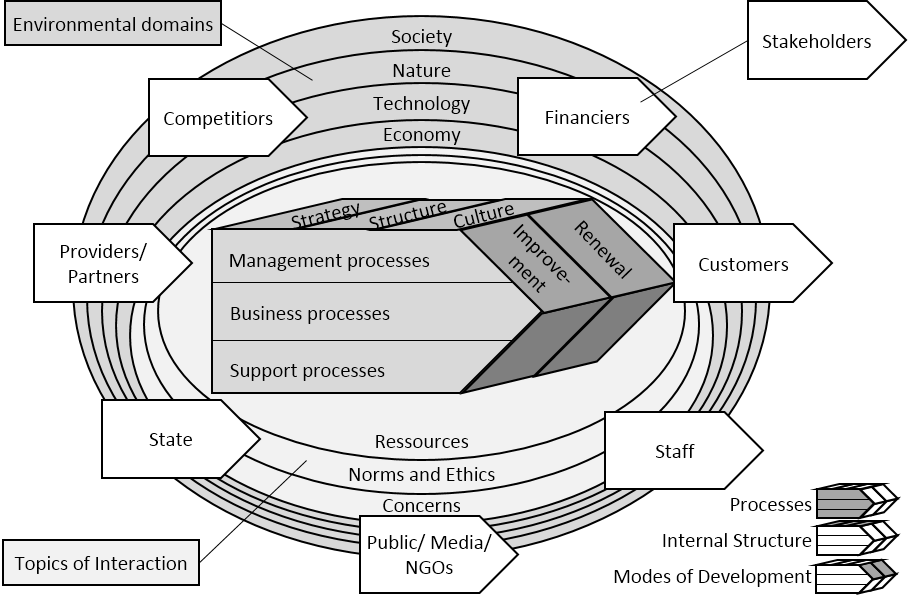
\includegraphics[width=1\textwidth]{img/SGM.png}
	\caption[St. Galler Management Modell]{The St. Galler Management Model from 2002 (own illustration based on \protect\cite{RueggSturm.2003})}
	\label{fig:SGM}
\end{figure}
The impact of this idea on the conception, which is the purpose of this paper, is that not only the direct customer of IBM and their decision makers must be analyzed for a sufficient planning of the application. The possible implication of the tendered project on the consumer and other stakeholder must become clear.
